%%%%%%%%%%%%%%%%%%%%%%%%%%%%%%%%%%%%%%%%%%%%%%%%%%%%%%%%%%%%%%%%%%%%%%%%%%%%%%%%
%%%%%%%%%%%%%%%%%%%%%%%%%%%%%%%%%%%%%%%%%%%%%%%%%%%%%%%%%%%%%%%%%%%%%%%%%%%%%%%%
\exercice{Représentation graphique d'un signal harmonique~\facile}
%%%%%%%%%%%%%%%%%%%%%%%%%%%%%%%%%%%%%%%%%%%%%%%%%%%%%%%%%%%%%%%%%%%%%%%%%%%%%%%%
%%%%%%%%%%%%%%%%%%%%%%%%%%%%%%%%%%%%%%%%%%%%%%%%%%%%%%%%%%%%%%%%%%%%%%%%%%%%%%%%
Soit un système linéaire du premier ordre régit par la fonction de 
transfert $H(p)$ telle que :
\[
H(p)=\dfrac{1}{1+2p}
\]
On considère la réponse harmonique à un signal d'entrée $e(t)=E_0\sin{\omega t}$
d'amplitude $E_0$ et de pulsation $\omega$.

On rappel (c.f annexe) que la réponse harmonique en régime permanent
à une telle sollicitation est de la forme :
\[
s(t)=E_0|H(\jw)|\sin{(\omega t+\phi)}\label{eq-rh}
\]
où $|H(\jw)|$ et $\phi(\omega)$ sont respectivement le module et 
l'argument du nombre complexe $H(\jw)$.
%%%%%%%%%%%%%%%%%%%%%%%%%%%%%%%%%%%%%%%%%%%%%%%%%%%%%%%%%%%%%%%%%%%%%%%%%%%%%%%%
\question{Déterminer le gain naturel $G(\omega)=|H(\jw)|$ et la 
phase $\phi(\omega)$ à partir de la fonction de transfert.}
%%%%%%%%%%%%%%%%%%%%%%%%%%%%%%%%%%%%%%%%%%%%%%%%%%%%%%%%%%%%%%%%%%%%%%%%%%%%%%%%
%%%%%%%%%%%%%%%%%%%%%%%%%%%%%%%%%%%%%%%%%%%%%%%%%%%%%%%%%%%%%%%%%%%%%%%%%%%%%%%%
\question{Tracer graphiquement la sollicitation $e(t)$ pour $E_0=1$, 
$\omega=\SI{1}{\radian\per\second}$ et  
$\omega=\SI{2}{\radian\per\second}$.} 
%%%%%%%%%%%%%%%%%%%%%%%%%%%%%%%%%%%%%%%%%%%%%%%%%%%%%%%%%%%%%%%%%%%%%%%%%%%%%%%%
%-------------------------------------------------------------------------------
%\begin{center}
%    \tikzsetnextfilename{sollicitation_harmonique-exercices-chap_repfreq-ext}
%    \input{tikz/sollicitation_harmonique-exercices-chap_repfreq.tex}
%\end{center}
%-------------------------------------------------------------------------------
%%%%%%%%%%%%%%%%%%%%%%%%%%%%%%%%%%%%%%%%%%%%%%%%%%%%%%%%%%%%%%%%%%%%%%%%%%%%%%%%
\question{Déterminer numériquement le gain et le déphasage pour  
$\omega=\SI{0.1}{\radian\per\second}$,  
$\omega=\SI{1}{\radian\per\second}$ et  $\omega=\SI{2}{\radian\per\second}$.}
%%%%%%%%%%%%%%%%%%%%%%%%%%%%%%%%%%%%%%%%%%%%%%%%%%%%%%%%%%%%%%%%%%%%%%%%%%%%%%%%
%%%%%%%%%%%%%%%%%%%%%%%%%%%%%%%%%%%%%%%%%%%%%%%%%%%%%%%%%%%%%%%%%%%%%%%%%%%%%%%%
\question{Tracer graphiquement la réponse harmonique avec la sollicitation 
pour $\omega=\SI{0.1}{\radian\per\second}$,   
$\omega=\SI{1}{\radian\per\second}$ et  
$\omega=\SI{2}{\radian\per\second}$. On choisira judicieusement l'échelle 
temporelle pour représenter une periode complète.}
%%%%%%%%%%%%%%%%%%%%%%%%%%%%%%%%%%%%%%%%%%%%%%%%%%%%%%%%%%%%%%%%%%%%%%%%%%%%%%%%
%-------------------------------------------------------------------------------
%\begin{center}
%    \tikzsetnextfilename{reponse1_harmonique-exercices-chap_repfreq-ext}
%    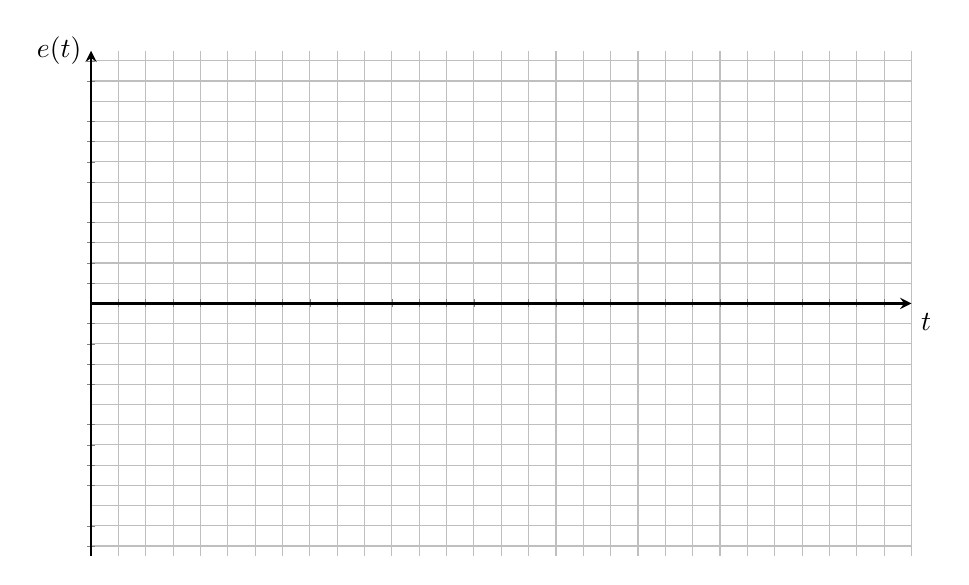
\begin{tikzpicture}
    \begin{axis}[
        ticks=none,
        axis line style = thick,
        height=8cm,
        width=12cm,
        axis x line=center,
        axis y line=center,
        xmin=0,
        xmax=120,
        ymin=-1.25,
        ymax=1.25,
        xlabel={$t$},
        ylabel={$e(t)$},
        xlabel style={below right},
        ylabel style={left},
        grid=both,
        minor tick num=4,
    ]
    \end{axis}
\end{tikzpicture}

%\end{center}
%-------------------------------------------------------------------------------
%-------------------------------------------------------------------------------
%\begin{center}
%    \tikzsetnextfilename{reponse2_harmonique-exercices-chap_repfreq-ext}
%    \input{tikz/reponse2_harmonique-exercices-chap_repfreq.tex}
%\end{center}
%-------------------------------------------------------------------------------
%-------------------------------------------------------------------------------
%\begin{center}
%    \tikzsetnextfilename{reponse3_harmonique-exercices-chap_repfreq-ext}
%    \input{tikz/reponse3_harmonique-exercices-chap_repfreq.tex}
%\end{center}
%-------------------------------------------------------------------------------
%\clearpage
%%%%%%%%%%%%%%%%%%%%%%%%%%%%%%%%%%%%%%%%%%%%%%%%%%%%%%%%%%%%%%%%%%%%%%%%%%%%%%%%
%%%%%%%%%%%%%%%%%%%%%%%%%%%%%%%%%%%%%%%%%%%%%%%%%%%%%%%%%%%%%%%%%%%%%%%%%%%%%%%%
\exercice{Diagramme de Bode~\moyen}
%%%%%%%%%%%%%%%%%%%%%%%%%%%%%%%%%%%%%%%%%%%%%%%%%%%%%%%%%%%%%%%%%%%%%%%%%%%%%%%%
%%%%%%%%%%%%%%%%%%%%%%%%%%%%%%%%%%%%%%%%%%%%%%%%%%%%%%%%%%%%%%%%%%%%%%%%%%%%%%%%
Tracer les diagrammes asymptotiques et réels de Bode des systèmes définis
par les fonctions de transfert suivantes :
%%%%%%%%%%%%%%%%%%%%%%%%%%%%%%%%%%%%%%%%%%%%%%%%%%%%%%%%%%%%%%%%%%%%%%%%%%%%%%%%
\question{}
%%%%%%%%%%%%%%%%%%%%%%%%%%%%%%%%%%%%%%%%%%%%%%%%%%%%%%%%%%%%%%%%%%%%%%%%%%%%%%%%
\[
H(p) = \dfrac{1}{10p+1}
\]
%%%%%%%%%%%%%%%%%%%%%%%%%%%%%%%%%%%%%%%%%%%%%%%%%%%%%%%%%%%%%%%%%%%%%%%%%%%%%%%%
\question{}
%%%%%%%%%%%%%%%%%%%%%%%%%%%%%%%%%%%%%%%%%%%%%%%%%%%%%%%%%%%%%%%%%%%%%%%%%%%%%%%%
\[
H(p) = \dfrac{100}{(10p+1)(100p+1)}
\]
%%%%%%%%%%%%%%%%%%%%%%%%%%%%%%%%%%%%%%%%%%%%%%%%%%%%%%%%%%%%%%%%%%%%%%%%%%%%%%%%
\question{}
%%%%%%%%%%%%%%%%%%%%%%%%%%%%%%%%%%%%%%%%%%%%%%%%%%%%%%%%%%%%%%%%%%%%%%%%%%%%%%%%
\[
H(p) = \dfrac{100(p+1)^2}{(100p+1)(10p+1)(0.01p+1)}
\]
%%%%%%%%%%%%%%%%%%%%%%%%%%%%%%%%%%%%%%%%%%%%%%%%%%%%%%%%%%%%%%%%%%%%%%%%%%%%%%%%
\question{}
%%%%%%%%%%%%%%%%%%%%%%%%%%%%%%%%%%%%%%%%%%%%%%%%%%%%%%%%%%%%%%%%%%%%%%%%%%%%%%%%
\[
H(p) = \dfrac{(10p+1)(0.1p+1)}{p(0.001p+1)^2}
\]
%%%%%%%%%%%%%%%%%%%%%%%%%%%%%%%%%%%%%%%%%%%%%%%%%%%%%%%%%%%%%%%%%%%%%%%%%%%%%%%%
\question{}
%%%%%%%%%%%%%%%%%%%%%%%%%%%%%%%%%%%%%%%%%%%%%%%%%%%%%%%%%%%%%%%%%%%%%%%%%%%%%%%%
\[
H(p) = \dfrac{10(10p+1)}{(p+1)(100p+1)}
\]
%%%%%%%%%%%%%%%%%%%%%%%%%%%%%%%%%%%%%%%%%%%%%%%%%%%%%%%%%%%%%%%%%%%%%%%%%%%%%%%%
%%%%%%%%%%%%%%%%%%%%%%%%%%%%%%%%%%%%%%%%%%%%%%%%%%%%%%%%%%%%%%%%%%%%%%%%%%%%%%%%
\exercice{Diagrammes de Nyquist~\difficile}
%%%%%%%%%%%%%%%%%%%%%%%%%%%%%%%%%%%%%%%%%%%%%%%%%%%%%%%%%%%%%%%%%%%%%%%%%%%%%%%%
%%%%%%%%%%%%%%%%%%%%%%%%%%%%%%%%%%%%%%%%%%%%%%%%%%%%%%%%%%%%%%%%%%%%%%%%%%%%%%%%
%%%%%%%%%%%%%%%%%%%%%%%%%%%%%%%%%%%%%%%%%%%%%%%%%%%%%%%%%%%%%%%%%%%%%%%%%%%%%%%%
\question{Tracer le diagramme de Nyquist de la fonction de transfert suivante:}
%%%%%%%%%%%%%%%%%%%%%%%%%%%%%%%%%%%%%%%%%%%%%%%%%%%%%%%%%%%%%%%%%%%%%%%%%%%%%%%%
\[
    H(p)=\dfrac{1}{p(p+1)}
\]
